\section{Architectural Decisions}
\label{se:architectural_decisions}

The initial design of \acrshort{wdias} used the \acrfull{soa}. Moreover, it tried to use an \acrfull{esb} to integrate different modules, as \acrshort{esb} could act as a shared layer for all of the modules to interact together. By default, \acrshort{esb} also provides publisher/subscriber capabilities.

The \acrshort{esb} processing units called \emph{mediators}. A mediator can take a message, carry out some predefined actions on it, and output the modified message. These mediator capabilities can be used to integrate the modules of a weather data system, as shown in \cref{fi:wdia_components}. \acrshort{esb} also supports different transportation protocols such as HTTP and web sockets. However, we realized that \acrshort{esb} is not suitable for data streaming or bulk data processing. Also, \acrshort{esb} suffers from a single point of failure, as all the messages are going through a common shared bus and slower communication (cannot be used for transfer data). In the second design phase of \acrshort{wdias}, we attempted to use the actor model using the AKKA framework \cite{HewittWhyModel} to overcome above \acrshort{esb} drawbacks. At the same time, we moved away from the \acrshort{soa} architecture design to the microservice architecture design.

Thus, we redesigned the system architecture with decomposing into microservices and used actors to implement each microservice in the system. In that case, we mapped each microservice in \acrshort{wdias} to an actor or an actor with slave actors. \acrshort{soa} focuses on imperative programming, while the microservices architecture focuses on a reactive actor programming style using faster messaging mechanisms.
When compared to \acrshort{soa}, the microservice architecture has several advantages:
\begin{itemize}
    \item Follow the principle of a single responsibility.
    \item Resilient/flexible because a failure of service does not influence other services. If you have monolithic or significant service errors in a service/module, this can have an impact on other modules/functionalities.
    \item High scalability because demanding services can be deployed on different servers to improve performance and stay away from other services so that they do not affect other services. It will be challenging to achieve the same with a single large monolithic service.
    \item Easy to improve the system because the microservices are decoupled from other services. It is also easier to change and test each microservices.
    \item Little impact on other services because each service is independent.
    \item Easy to understand because they represent a small functionality.
    \item Ease of deployment.
\end{itemize}

The AKKA framework has some of the disadvantages of implementing each microservice as an actor, as described in AKKA documentation \cite{Akka.ioWhenCluster}. One of the attractive features of microservice architecture is the independent nature of the microservices. The above concept allows choosing different technologies for each microservice based on the advantage that could bring in. Also, the microservice architecture will enable us to independently develop and maintain a system by multiple smaller and more focused teams/communities. But using the actors as microservice, the actors communicate using message passing cause to result in a too-tight code coupling between the services and difficulty to deploy services independent of each other, which is one of the main reasons for using a microservices architecture \cite{Akka.ioWhenCluster}. To overcome these problems, we moved to the concept of container orchestration based microservice architecture.

Containerization is an alternative to virtualization that supports virtual machines or hypervisors. It includes encapsulating or grouping the software code and all its dependencies so that it can work uniformly and consistently in any infrastructure \cite{IBMContainerizationExplained}. The concept of containerization and process isolation has emerged after the open source Docker Engine \cite{DockerAppContainerization}, an industry standard for package software into standardized units for development, shipment, and deployment.

The \acrshort{wdias} used \acrfull{k8s} as the container orchestration system. \acrshort{k8s} is an open-source tool for automating deployment, scaling, and management of containerized applications [15]. It groups the containers that make up an application into logical units for easy management and detection. Using \acrshort{k8s}, we deploy each microservice as a container and manage it by providing scalability and availability.

\begin{figure}[htp]
    \centering
    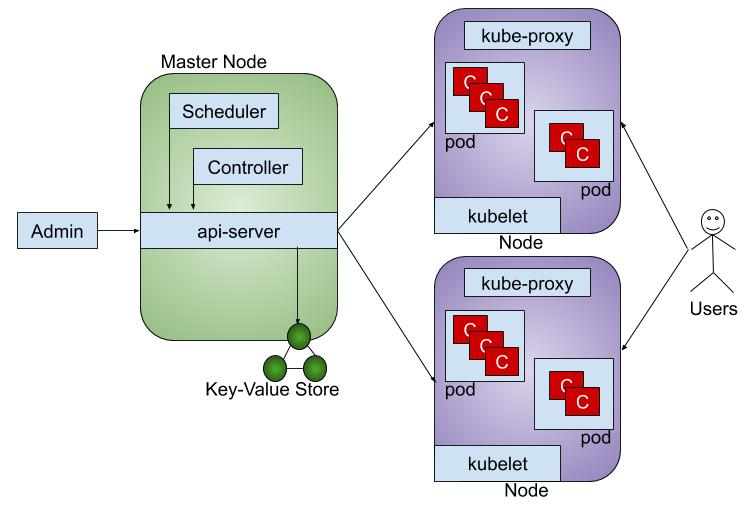
\includegraphics[width=1\textwidth]{method/microservice/k8s_architecture_v3.jpg}
    \caption{\acrfull{k8s} architecture.}
    \label{fi:k8s_architecture}
\end{figure}

\cref{fi:k8s_architecture} give an overall idea on the components of \acrshort{k8s},
\begin{itemize}
    \item Pods -- Cluster of containers that can group other container images in a single unit.
    \item Nodes -- The machines (VMs, physical servers, etc) in a cluster that runs your applications and cloud workflows.
    \item Kubelet -- An agent that runs on each node in the cluster. It makes sure that containers are running in a pod.
    \item Kube-proxy -- A network proxy that runs on each node in the cluster, and maintains network rules on nodes.
    \item Kubernetes master -- Responsible for maintaining the desired state for your cluster.
    \item etcd -- Consistent and highly-available key value store used as \acrshort{k8s} backing store for all cluster data.
\end{itemize}

Users can add nodes much as required into the \acrshort{k8s} cluster, and \acrshort{k8s} manage and deploy applications as pods into cluster nodes. Each microservice can deploy as a pod, which is a group of containerized applications. \acrshort{k8s} is able to scale as much as the user requirements by deploying multiple copies of the same pod. By separating each microservice as a container, and running them as multiple pods inside the \acrshort{k8s} removes the tight coupling of microservices when compared to the actors. It preserves the independent nature of the microservices and supports the high scalability of the system.

%%%%%%%%%%%%%%%%%%%%%%%%%%%%%%%%%%%%%%%%%%%%%%%%%%%%%%%%%%%%%%%%%%%%%%%%%%%%%%%%
% Architecture Comparison with Existing Systems

\begin{figure}[htp]
    \centering
    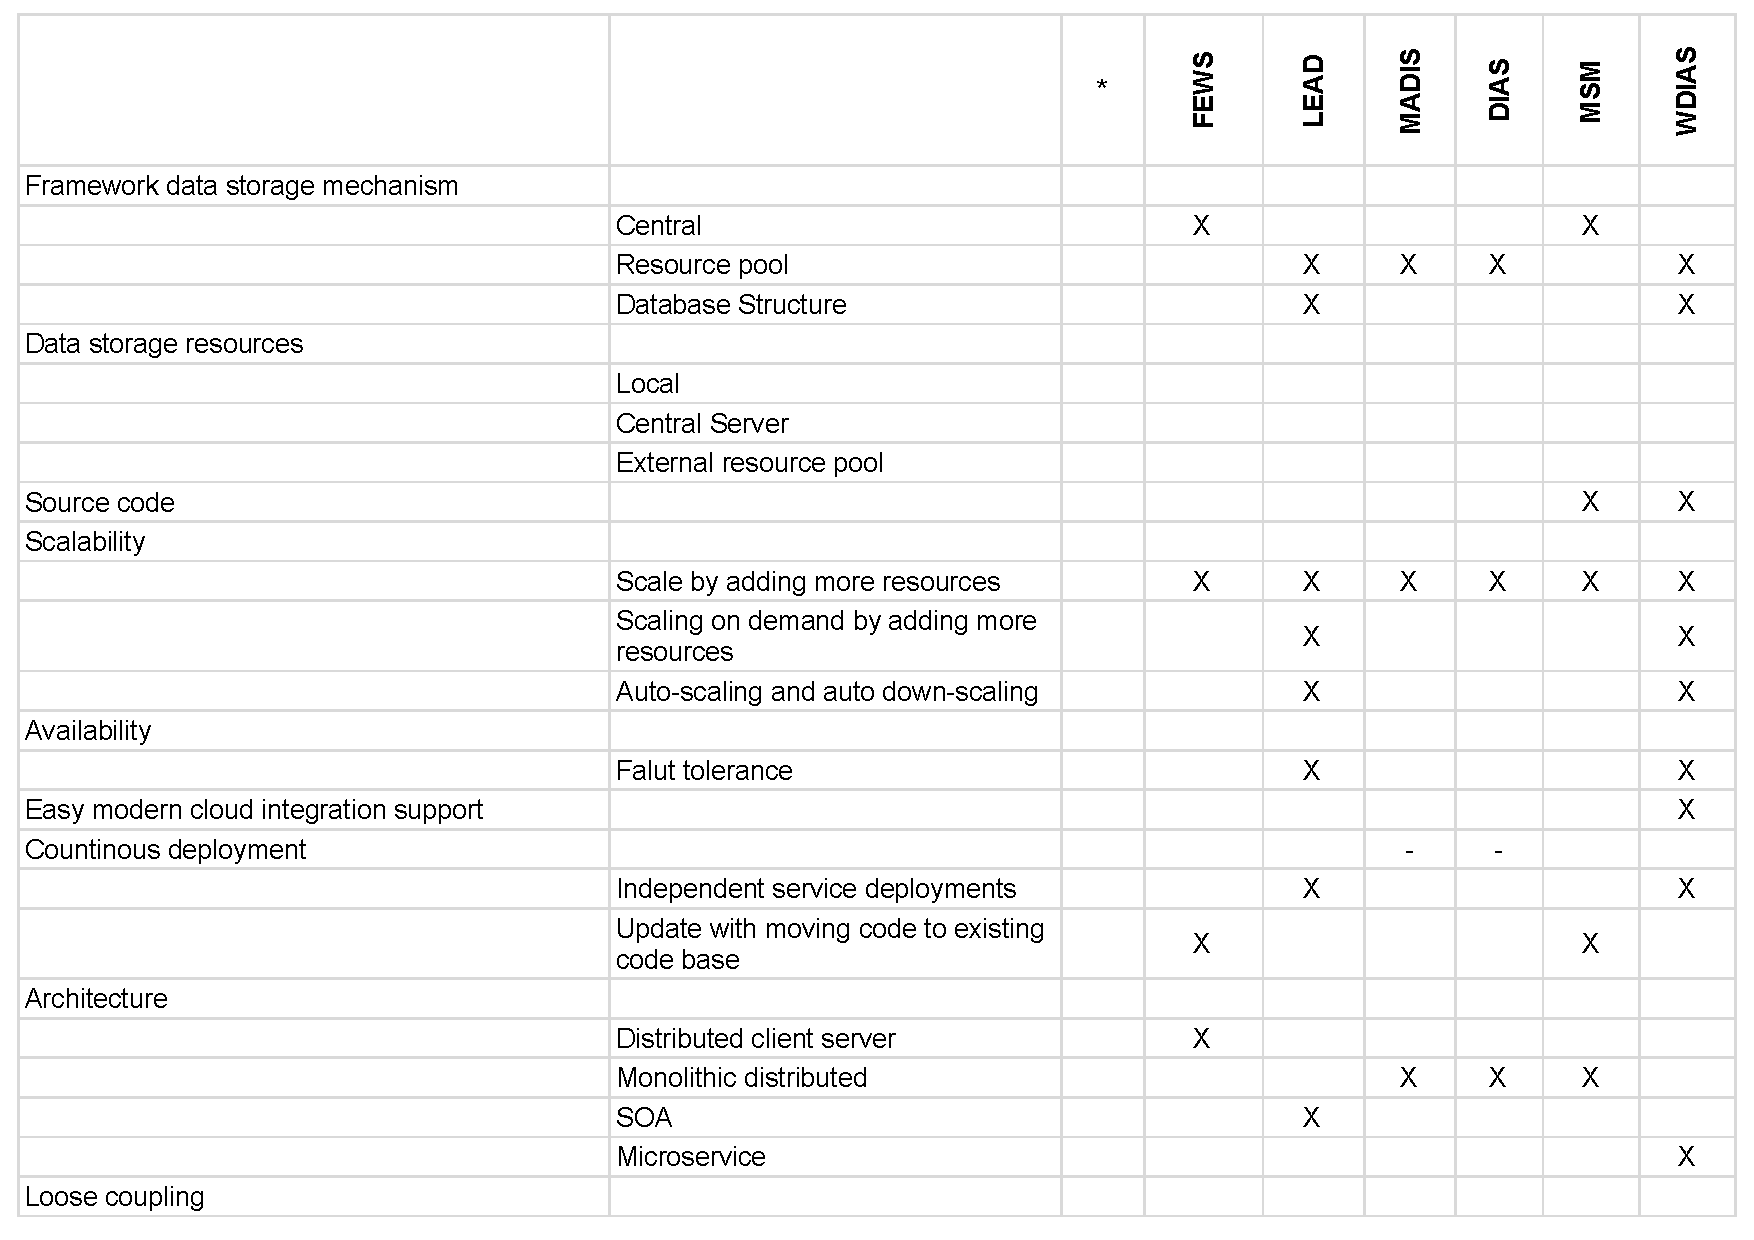
\includegraphics[width=1.05\textwidth]{method/misc/architecture_comparison_pros_cons.pdf}
    \caption{Comparison of available features among existing weather data assimilation and integration systems and \acrshort{wdias}. An "X" in the table represents a feature offered by the corresponding tool. An "-" in the table represents that information available are not enough to make an statement, and empty presents a feature is not offered. }
    \label{fi:architecture_comparison}
\end{figure}

\gc{\cref{fi:architecture_comparison} shows a summarized architecture comparison between existing systems that we discussed in the WDIAS. Here, we analyze the systems under a few categories such as data resources of the system, performance, architecture of the system, and other available main features. The fews and msm frameworks store the data through a central data service which can be a bottleneck handling large amounts of data in a critical situation. Other systems are capable of using a resource pool which allows them to grow the performance while adding more resources to the system.  Regarding the performance of the systems, we consider scalability, availability, cloud computing support, and system deployment capabilities. All of the systems are capable of scaling up to some extent by adding resources beforehand or in real time. But the LEAD, DIAS and WDIAS are capable of scaling on demand by adding more resources, and also support auto scaling up and scaling down. The LEAD, MADIS, DIAS and WDIAS able to provide availability, since those were able to run using a resource pool which can run on different locations, and systems are capable of automatically handling partial system failures, hence supporting fault tolerance. When we discuss about the modern cloud computing support, the system should support easy integration with clouds. It is possible to rent virtual servers and deploy the local services in the cloud infrastructure, but some systems may not allow access to them remotely. Even some systems able to deploy in such manner, they may not be capable of automatically resource allocation on demand. Hence, we can not consider that those systems are full cloud infrastructures. Furthermore, we can easily maintain a system if it consists of independent subsystems, and each subsystem is capable of deploying or upgrading independently. Independent service deployment is a more flexible and better way to handle this, rather than copy pasting codes in order to deploy changes.}

\gc{We discuss the architecture of the systems in their pattern, dependencies of the subsystems, extendable with adding more features easily, source code availability, and data preprocessing capabilities specific to the weather domain. While other existing systems are using distributed client server architecture or monolithic distributed architecture, LEAD is using the SOA architecture, but WDIAS has the more advantage of using modern cloud computing technologies with implementing microservices as containerized applications. The architecture implementation of independent subsystems allow users to maintain subsystems independently. Further, WDIAS allow to use own technology stack for each subsystem with using different programming languages. Specially the WDIAS and MSM provide open source framework which gives the capability for users to enhance or modify the system as per the requirement. All of these systems provide data preprocessing capabilities for weather data, and adding new preprocessing capabilities. But WDIAS is capable of providing auto scaling with data preprocessing as well. Workflow engine and model execution support are some other extra features that are helpful with weather forecasting. But the WDIAS focus is about implementing a WDIA system with supporting main features, and it provides an extendable open framework to integrate such features easily.}
